% !TeX root = ./memoria.tex
%%%%%%%%%%%%%%%%%%%%%%%%%%%%%%%%%%%%%%%%%
% Masters/Doctoral Thesis 
% LaTeX Template
% Version 2.3 (25/3/16)
%
% This template has been downloaded from:
% http://www.LaTeXTemplates.com
%
% Version 2.x major modifications by:
% Vel (vel@latextemplates.com)
%
% This template is based on a template by:
% Steve Gunn (http://users.ecs.soton.ac.uk/srg/softwaretools/document/templates/)
% Sunil Patel (http://www.sunilpatel.co.uk/thesis-template/)
%
% Template license:
% CC BY-NC-SA 3.0 (http://creativecommons.org/licenses/by-nc-sa/3.0/)
%
%%%%%%%%%%%%%%%%%%%%%%%%%%%%%%%%%%%%%%%%%

%----------------------------------------------------------------------------------------
%	PACKAGES AND OTHER DOCUMENT CONFIGURATIONS
%----------------------------------------------------------------------------------------

\documentclass[
11pt, % The default document font size, options: 10pt, 11pt, 12pt
%oneside, % Two side (alternating margins) for binding by default, uncomment to switch to one side
%chapterinoneline,% Have the chapter title next to the number in one single line
%english, % ngerman for German
spanish,
singlespacing, % Single line spacing, alternatives: onehalfspacing or doublespacing
%draft, % Uncomment to enable draft mode (no pictures, no links, overfull hboxes indicated)
%nolistspacing, % If the document is onehalfspacing or doublespacing, uncomment this to set spacing in lists to single
%liststotoc, % Uncomment to add the list of figures/tables/etc to the table of contents
%toctotoc, % Uncomment to add the main table of contents to the table of contents
parskip, % Uncomment to add space between paragraphs
%nohyperref, % Uncomment to not load the hyperref package
headsepline, % Uncomment to get a line under the header
]{MastersDoctoralThesis} % The class file specifying the document structure



%----------------------------------------------------------------------------------------
%	INFORMACIÓN DE LA MEMORIA
%----------------------------------------------------------------------------------------

\thesistitle{Firmware para robot de navegación autónoma} % El títulos de la memoria, se usa en la carátula y se puede usar el cualquier lugar del documento con el comando \ttitle
\degree{Especialista en Sistemas Embebidos } % Nombre del grado, se usa en la carátula y se puede usar el cualquier lugar del documento con el comando \degreename
\author{Ing. Alexis Martin Pojomovsky} % Tu nombre, se usa en la carátula y se puede usar el cualquier lugar del documento con el comando \authorname
\supervisor{Dr. Pablo De Cristóforis (FCEyN-UBA)} % El nombre del director, se usa en la carátula y se puede usar el cualquier lugar del documento con el comando \supname
\juradoUNO{Esp. Ing. Diego Fernández (FI-UBA)} % Nombre y pertenencia del un jurado se usa en la carátula y se puede usar el cualquier lugar del documento con el comando \jur1name
\juradoDOS{Esp. Ing. Edgardo Comas (CITEDEF/UTN-FRBA)} % Nombre y pertenencia del un jurado se usa en la carátula y se puede usar el cualquier lugar del documento con el comando \jur2name
\juradoTRES{Esp. Ing. Gerardo Puga (UNLP)} % Nombre y pertenencia del un jurado se usa en la carátula y se puede usar el cualquier lugar del documento con el comando \jur3name
\fechaINICIO{enero de 2018}
\fechaFINAL{agosto de 2020}

\subject{Memoria del Trabajo Final de la Carrera de Especialización en Sistemas Embebidos de la UBA} % Your subject area, this is not currently used anywhere in the template, print it elsewhere with \subjectname
\keywords{Sistemas Embebidos, CESE, FIUBA} % Keywords for your thesis, this is not currently used anywhere in the template, print it elsewhere with \keywordnames
\university{Universidad de Buenos Aires} % Your university's name and URL, this is used in the title page and abstract, print it elsewhere with \univname
\faculty{{Facultad de Ingeniería}} % Your faculty's name and URL, this is used in the title page and abstract, print it elsewhere with \facname
\department{Departamento de Electrónica} % Your department's name and URL, this is used in the title page and abstract, print it elsewhere with \deptname
\group{{Laboratorio de Sistemas Embebidos}} % Your research group's name and URL, this is used in the title page, print it elsewhere with \groupname


%\hypersetup{pdftitle=\ttitle} % Set the PDF's title to your title
%\hypersetup{pdfauthor=\authorname} % Set the PDF's author to your name
%\hypersetup{pdfkeywords=\keywordnames} % Set the PDF's keywords to your keywords


%\newcaptionname{spanish}{\acknowledgementname}{Agradecimientos}
%\newcaptionname{spanish}{\authorshipname}{Declaración de Autoría}
%\newcaptionname{spanish}{\abbrevname}{Glosario}
%\newcaptionname{spanish}{\byname}{por}
%
%\renewcommand{\lstlistingname}{Código}% Listing -> Algorithm
%\renewcommand{\lstlistlistingname}{Índice de \lstlistingname s}% List of Listings -> List of Algorithms
%
%\renewcommand{\listtablename}{Índice de Tablas}
%\renewcommand{\tablename}{Tabla} 

\addtolength{\footnotesep}{2mm} % Espacio adicional en los footnotes

\begin{document}

\frontmatter % Use roman page numbering style (i, ii, iii, iv...) for the pre-content pages

\pagestyle{plain} % Default to the plain heading style until the thesis style is called for the body content

%----------------------------------------------------------------------------------------
%	CARÁTULA
%----------------------------------------------------------------------------------------

\begin{titlepage}
\begin{center}


\includegraphics[width=.8\textwidth]{./Figures/logoFIUBA.png}
\vspace{2cm}

\textsc{\huge{Carrera de Especialización en\\ \vspace{5px} Sistemas Embebidos}}
\vspace{.5cm} % Thesis type

\textsc{\Large Memoria del Trabajo Final}\\[1cm] % Thesis type
%\vspace{1.5cm}
{\huge \bfseries \ttitle\par}\vspace{0.4cm} % Thesis title

\vfill

\vspace{1.5cm}
\LARGE\textbf{Autor:\\
\authorname}\\ % Author name

\vspace{1.5cm}

\large
{Director:} \\
{\supname} % Supervisor name
 
\vspace{1cm}
Jurados:\\	
\jurunoname\\
\jurdosname\\
\jurtresname

\vspace{2cm}

\textit{Este trabajo fue realizado en las Ciudad Autónoma de Buenos Aires,\\ entre \fechaINICIOname \hspace{1px} y \fechaFINALname.}
\end{center}
\end{titlepage}


%----------------------------------------------------------------------------------------
%	RESUMEN - ABSTRACT 
%----------------------------------------------------------------------------------------

\begin{abstract}
\addchaptertocentry{\abstractname} % Add the abstract to the table of contents
%
%The Thesis Abstract is written here (and usually kept to just this page). The page is kept centered vertically so can expand into the blank space above the title too\ldots
\centering

La presente memoria describe el desarrollo del robot móvil ``Lubobot``, destinado a entornos educativos de grado universitario a través de las distintas etapas de estudio de la materia ``Robótica Móvil``, dictada como materia de la carrera de Ingeniería Mecatrónica en la Universidad Nacional de Asunción, Paraguay. Como parte del trabajo se realizó la implementación básica requerida para utilizar este robot con el Sistema Operativo Robótico (ROS).

Se aplicaron diversos conocimientos adquiridos durante la carrera, entre los que se destacan los referidos a sistemas operativos, control de versiones y protocolos de comunicación. Así también, se hicieron uso de patrones de diseño y técnicas de modularización de software.

\end{abstract}

%----------------------------------------------------------------------------------------
%	CONTENIDO DE LA MEMORIA  - AGRADECIMIENTOS
%----------------------------------------------------------------------------------------

\begin{acknowledgements}
%\addchaptertocentry{\acknowledgementname} % Descomentando esta línea se puede agregar los agradecimientos al índice
\vspace{1.5cm}

Agradezco el apoyo provisto por mi esposa Laura así como el de mis padres Evelyn y Ernesto, presentes durante todo el proceso de mi formación, siempre alentándome a ir un paso mas allá.\\
Al equipo docente y colaboradores de la Carrera de Especialización de Sistemas Embebidos, por la dedicación y entrega manifestados durante cada etapa de la cursada.

\end{acknowledgements}

%----------------------------------------------------------------------------------------
%	LISTA DE CONTENIDOS/FIGURAS/TABLAS
%----------------------------------------------------------------------------------------
\renewcommand{\listtablename}{Índice de Tablas}

\tableofcontents % Prints the main table of contents
%
\listoffigures % Prints the list of figures
%
\listoftables % Prints the list of tables

%----------------------------------------------------------------------------------------
%	CONTENIDO DE LA MEMORIA  - CAPÍTULOS
%----------------------------------------------------------------------------------------

\mainmatter % Begin numeric (1,2,3...) page numbering

\pagestyle{thesis} % Return the page headers back to the "thesis" style

%\renewcommand{\tablename}{Tabla} %TODO eliminar esta línea

% Incluir los capítulos como archivos separados desde la carpeta Chapters
% Descomentar las líneas a medida que se escriben los capítulos

% !TEX root = ../memoria.tex

\chapter{Introducción general}

\label{Chapter1}

En este capítulo se introduce el campo de estudio de la robótica móvil y la importancia de una planta de pruebas física como motivación para la realización de este trabajo. Asimismo, se presentan los objetivos y el alcance del presente proyecto.

%----------------------------------------------------------------------------------------
%	SECTION 1
%----------------------------------------------------------------------------------------

\section{Motivación}

La robótica de manipuladores, también llamados brazos robóticos, se han ganado su puesto como ciudadanos de primera clase en la industria de la manufactura. Difícilmente podríamos al día de hoy, imaginarnos una planta de fabricación en serie que no disponga de estos dispositivos para la realización de tareas repetitivas y de alta precisión.

En la industria electrónica, por citar un ejemplo, los manipuladores son capaces de colocar componentes de montaje superfical con una precisión y velocidad por lejos sobre-humana, haciendo posible la elaboración de teléfonos celulares, computadoras portátiles, etc.
Sin embargo, y a pesar de su innegable éxito, estos robots sufren de una desventaja particular: la falta de movilidad. Un manipulador fijo posee un rango de movimiento limitado que depende del sitio en que el mismo se encuentre instalado. Por el contrario, un robot móvil sería capaz de moverse a través de la planta, permitiendo el aprovechamiento de sus facultades donde sea que estas sean precisadas.

La robótica móvil responde a la pregunta de "¿cómo moverse desde un determinado punto en el espacio a otro atravezando un entorno impredecible y sin supervisión?". Si bien la respuesta a esta pregunta podría resultar casi trivial si se tratase de un protagonista humano, la realidad es que representa un desafío mayor para un robot y por ello existe una rama completa de estudios dedicada a ella.

El estudio de la robótica en las universidades argentinas se encuentra mayormente avocada a la robótica de manipuladores. Esto tiene sentido desde un punto de vista de oferta/demanda en la industria local, sin embargo, el mercado internacional esta viviendo una fuerte demanda de profesionales capaces de entender y aplicar técnicas de robótica móvil.

Considerando que hasta hace solo unos años atrás los sensores y computadoras requeridos para estas tareas tenían costos altamente prohibitivos.
El estudio de robótica móvil es tan importante como el de la robótica de manipuladores.

Diversas empresas han adoptado este desafío y se encuentran, al día de hoy, trabajando en soluciones con robots móviles.
Los vehículos autónomos son un ejemplo de ello, 

\todo {Terminar la motivación}

%-----------------------------------
%	SUBSECTION 1
%-----------------------------------
\subsection{Subsection 1}

Nunc posuere quam at lectus tristique eu ultrices augue venenatis. Vestibulum ante ipsum primis in faucibus orci luctus et ultrices posuere cubilia Curae; Aliquam erat volutpat. Vivamus sodales tortor eget quam adipiscing in vulputate ante ullamcorper. Sed eros ante, lacinia et sollicitudin et, aliquam sit amet augue. In hac habitasse platea dictumst.

%-----------------------------------
%	SUBSECTION 2
%-----------------------------------

\subsection{Subsection 2}
Morbi rutrum odio eget arcu adipiscing sodales. Aenean et purus a est pulvinar pellentesque. Cras in elit neque, quis varius elit. Phasellus fringilla, nibh eu tempus venenatis, dolor elit posuere quam, quis adipiscing urna leo nec orci. Sed nec nulla auctor odio aliquet consequat. Ut nec nulla in ante ullamcorper aliquam at sed dolor. Phasellus fermentum magna in augue gravida cursus. Cras sed pretium lorem. Pellentesque eget ornare odio. Proin accumsan, massa viverra cursus pharetra, ipsum nisi lobortis velit, a malesuada dolor lorem eu neque.

%----------------------------------------------------------------------------------------
%	SECTION 2
%----------------------------------------------------------------------------------------

\section{Descripción de tecnologías}

Sed ullamcorper quam eu nisl interdum at interdum enim egestas. Aliquam placerat justo sed lectus lobortis ut porta nisl porttitor. Vestibulum mi dolor, lacinia molestie gravida at, tempus vitae ligula. Donec eget quam sapien, in viverra eros. Donec pellentesque justo a massa fringilla non vestibulum metus vestibulum. Vestibulum in orci quis felis tempor lacinia. Vivamus ornare ultrices facilisis. Ut hendrerit volutpat vulputate. Morbi condimentum venenatis augue, id porta ipsum vulputate in. Curabitur luctus tempus justo. Vestibulum risus lectus, adipiscing nec condimentum quis, condimentum nec nisl. Aliquam dictum sagittis velit sed iaculis. Morbi tristique augue sit amet nulla pulvinar id facilisis ligula mollis. Nam elit libero, tincidunt ut aliquam at, molestie in quam. Aenean rhoncus vehicula hendrerit.


%----------------------------------------------------------------------------------------
%	SECTION 3
%----------------------------------------------------------------------------------------

\section{Objetivos y alcance}

Sed ullamcorper quam eu nisl interdum at interdum enim egestas. Aliquam placerat justo sed lectus lobortis ut porta nisl porttitor. Vestibulum mi dolor, lacinia molestie gravida at, tempus vitae ligula. Donec eget quam sapien, in viverra eros. Donec pellentesque justo a massa fringilla non vestibulum metus vestibulum. Vestibulum in orci quis felis tempor lacinia. Vivamus ornare ultrices facilisis. Ut hendrerit volutpat vulputate. Morbi condimentum venenatis augue, id porta ipsum vulputate in. Curabitur luctus tempus justo. Vestibulum risus lectus, adipiscing nec condimentum quis, condimentum nec nisl. Aliquam dictum sagittis velit sed iaculis. Morbi tristique augue sit amet nulla pulvinar id facilisis ligula mollis. Nam elit libero, tincidunt ut aliquam at, molestie in quam. Aenean rhoncus vehicula hendrerit.

% !TeX root = ./../memoria.tex
\chapter{Introducción específica}

\label{Capitulo2}

En este capítulo se desglosan las diferentes herramientas tanto de hardware como de software elegidas para el desarrollo del robot propuesto.

\section{Robot Operating System}

Comúnmente denominado ROS, es un framework de robótica de código abierto que fue diseñado originalmente para robots de uso académico. Sin embargo, al día de hoy su uso se ha extendido tanto a la industria como al público aficionado.

ROS ofrece un variado \textit{set} de herramientas que facilitan las tareas del roboticista en funciones como envío y recepción de mensajes, computación distribuida e implementación de algoritmos para aplicaciones robóticas.

\subsection{Organización de archivos}\label{sec:organizacionArchivos}

Es adecuado considerar a ROS como algo más que un framework de desarrollo y referirnos a el como un ``meta sistema operativo'', ya que ofrece no solo herramientas y bibliotecas sino también funciones similares a las de un sistema operativo. Entre ellas, podemos citar su abstracción del hardware, el manejo de paquetes, además de un completo \textit{toolchain} de compilación. Así también, tal como en un sistema operativo ``real'', los archivos que componen ROS se encuentran organizados en el disco duro de una manera particular, como se indica en la figura \ref{fig:rosSistemaDeArchivos}.

\begin{figure}[ht]
    \centering
    \def\svgwidth{350pt}
    \input{./Figures/estructura_archivos_ros.pdf_tex}
    \caption{Organización de archivos en ROS}
    \label{fig:rosSistemaDeArchivos}
\end{figure}

\newpage
A continuación se detalla en qué consiste cada uno de los bloques que componen la organización de archivos:
\begin{itemize}
    \item \textbf{Paquetes}: los paquetes de ROS representan la unidad básica de software en la plataforma. Contienen uno o más programas de ROS (nodos), bibliotecas, archivos de configuración, etc, que son organizados como una unidad coherente.
    \item \textbf{Manifiesto del paquete}: está representado por un archivo único dentro del paquete que contiene información sobre este tales como el nombre, autor, tipo de licencia, dependencias, banderas de compilación, etc. El archivo \file{package.xml} encontrado en la raíz del paquete es su propio manifiesto.
    \item \textbf{Metapaquete}: hace referencia a uno o más paquetes usualmente relacionados entre sí, pero sin estar necesariamente acoplados fuertemente unos con otros. El software provisto con este proyecto es un metapaquete.
    \item \textbf{Manifiesto del metapaquete}: similar al manifiesto del paquete, con la diferencia que este puede incluir dependencias a de tiempo de ejecución hacia otros paquetes.
    \item \textbf{Mensajes}: representados con la extensión \file{.msg}, son los tipos de datos utilizados por ROS internamente para comunicar los distintos procesos entre sí. El usuario puede definir tipos de mensajes personalizados con campos adaptados a sus necesidades en del directorio \file{msg} dentro del paquete.
    \item  \textbf{Servicios}: representados con la extensión \file{.srv}, representan interacciones del tipo solicitud/respuesta entre distintos procesos. Los formatos tanto para solicitud como para respuesta pueden definirse en el directorio \file{srv} dentro del paquete.
    \item \textbf{Repositorios}: la gran mayoría de los paquetes de ROS son mantenidos utilizando un sistema de control de versiones (SCV) tales como Git, Mercurial o SVN. Es común encontrar metapaquetes definidos dentro de un mismo único repositorio. Este es el caso para el repositorio provisto en este trabajo.
\end{itemize}

\subsection{Arquitectura interna}
ROS está construido sobre una arquitectura basada en grafos, esto significa que las tareas de cómputo son realizadas a través de una red de procesos llamados nodos. Esta red es denominada \textit{Computation Graph} o grafo de cómputo.

Los principales componentes de este grafo son los nodos, el \textit{master} o maestro, el \textit{parameter server} o servidor de parámetros, además de los mensajes, tópicos, servicios y \textit{bags} o bolsas. Cada uno de estos elementos contribuye al funcionamiento del \textit{Computation Graph} con una funcionalidad específica. Los elementos que lo componen, mostrados en la figura \ref{fig:computationGraph}, se describen a continuación:

\newpage

\begin{figure}[ht]
    \centering
    \def\svgwidth{350pt}
    \input{./Figures/ros_computation_graph.pdf_tex}
    \caption{Estructura del \textit{Computation Graph} de ROS.}
    \label{fig:computationGraph}
\end{figure}

\begin{itemize}
    \item \textbf{Nodos}: son los procesos que realizan las tareas de cómputo dentro del robot, que pueden comunicarse unos con otros a través de la API de ROS. Esto resulta particularmente útil cuando distintos nodos necesitan compartir información entre sí. En ROS se fomenta el uso de múltiples nodos que realicen procesos sencillos por sobre procesos grandes y complejos que abarquen toda la funcionalidad.
    \item \textbf{Master}: el ROS Master se encarga de buscar y registrar los diferentes componentes que interactúan en el sistema. Esto posibilita que diferentes nodos sean capaces de ``encontrarse'' mutuamente, intercambiar mensajes o invocar servicios. En un sistema distribuido, el master debe ejecutarse solamente en una de las computadoras.
    \item \textbf{Servidor de parámetros}: el servidor de parámetros o \textit{parameter server}, permite mantener la información utilizada en configuración de los nodos almacenada en una ubicación central. Esto permite a cada uno de los nodos a acceder y modificar dichos valores.
    \item \textbf{Mensajes}: los nodos se comunican entre sí mediante mensajes, estructuras de datos cuyos campos pueden editarse y permiten ser enviados entre sí. Existen tipos de mensajes estándares (enteros, flotantes, booleanos, etc.) así como también es posible definir mensajes propios, adaptados a las necesidades de la aplicación.
    \item \textbf{Tópicos}: cada mensaje en ROS es transportado utilizando buses llamados tópicos. Cuando un nodo envía un mensaje a través de un tópico, se puede decir que el nodo está ``publicando un tópico''. Asimismo cuando un nodo recibe un mensaje a través de un tópico, se puede decir que el nodo está ``subscripto al tópico''. El nodo publicante y el suscriptor no tienen información sobre su mutua existencia, por lo que es posible que existan nodos que publiquen en tópicos sin suscriptores o viceversa, es decir nodos suscriptos a tópicos sin publicantes.
    \item \textbf{Servicios}: en determinadas aplicaciones, el mecanismo de publicador/suscriptor definido en el ítem anterior podría no ser adecuado. Por ejemplo, en ciertos casos es necesaria una interacción del tipo solicitud/respuesta. En dichas situaciones un nodo podría solicitar la ejecución de un procedimiento rápido por parte de otro nodo y el envío de una respuesta con el resultado de dicho cálculo.
    \item \textbf{Logging}: ROS provee un sistema de registro o \textit{logging} denominado rosbag (bolsa), que se utiliza para almacenar información publicada en los tópicos activos, como por ejemplo la proveniente de un sensor que podría ser difícil de generar una y otra vez, pero que a su vez resulta necesaria para depurar determinados algoritmos. Un rosbag permitiría en este caso generar la información una única vez para luego reproducirla como si fuese una grabación las veces que resulte necesario.
\end{itemize}

\subsection{Herramienta RViz}

La herramienta RViz (o ROS Visualization tool) es la herramienta oficial de visualización ROS, que permite representar de manera gráfica la información transmitida a través de los distintos tópicos. Posee soporte nativo para la mayoría de los mensajes estándar y permite además, expandir su funcionamiento mediante \textit{plugins} que posiblitan entre otras cosas, visualizar mensajes definidos por el usuario. La configuración estándar de RViz permite visualizar la configuración de articulaciones (o \textit{joints}) y enlaces (o \textit{links}) de un robot como se muestra en la figura \ref{fig:rviz}.

\begin{figure}[ht]
    \centering
    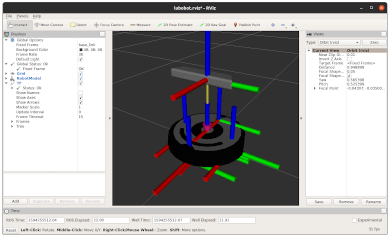
\includegraphics{./Figures/rviz.png}
    \caption{Interfaz gráfica de RViz donde se muestran los \textit{links} y \textit{joints} del robot Lubobot.}
    \label{fig:rviz}
\end{figure}


\subsection{Formato universal de descripción de robots URDF}

El formato universal de descripción de robots o \textit{Universal Robot Description System}, comúnmente referido como URDF es un formato estándar para representación de modelos conformados por múltiples piezas conectadas entre sí, como es el caso de brazos robóticos o líneas de ensamblaje. Este es ampliamente utilizado dentro del ecosistema de ROS, plataforma donde vio su origen aunque al día de hoy su uso se ha extendido a herramientas externas como MATLAB, que permite importar archivos URDF directamente a su \textit{toolbox} de robótica.

\subsection{Biblioteca rosserial}\label{sec:rosserial}

Es un protocolo para la transmisión serial de mensajes y multiplexación de múltiples tópicos y servicios de ROS sobre un \textit{character device} tal como un puerto UART o un \textit{socket} de red.
Además de la definición del protocolo de serialización en si mismo, rosserial se compone de otros dos elementos principales:
\begin{itemize}
    \item \textbf{bibliotecas cliente}: permiten la integración de nodos ROS en diferentes plataformas, apuntando principalmente a sistemas embebidos. Dichas librerias son especializaciones de una clase base, escrita en ANSI C++ para mayor compatiblidad y denominada rosserial\_client. Para este trabajo se realizó un \textit{port} de dicha biblioteca a la plataforma STM32CubeHAL.
    \item \textbf{Interfaz con ROS}: las bibliotecas cliente requieren de que haya un nodo corriendo en la computadora \textit{host} que funcione como puente entre el serie y la red de ROS, que se encarga de des-serializar y serializar los mensajes que llegan y se despachan, respectivamente. La participación de los distintos actores involucrados en el uso de rosserial se muestran en la figura \ref{fig:rosserial}.
\end{itemize}

\begin{figure}[ht]
    \centering
    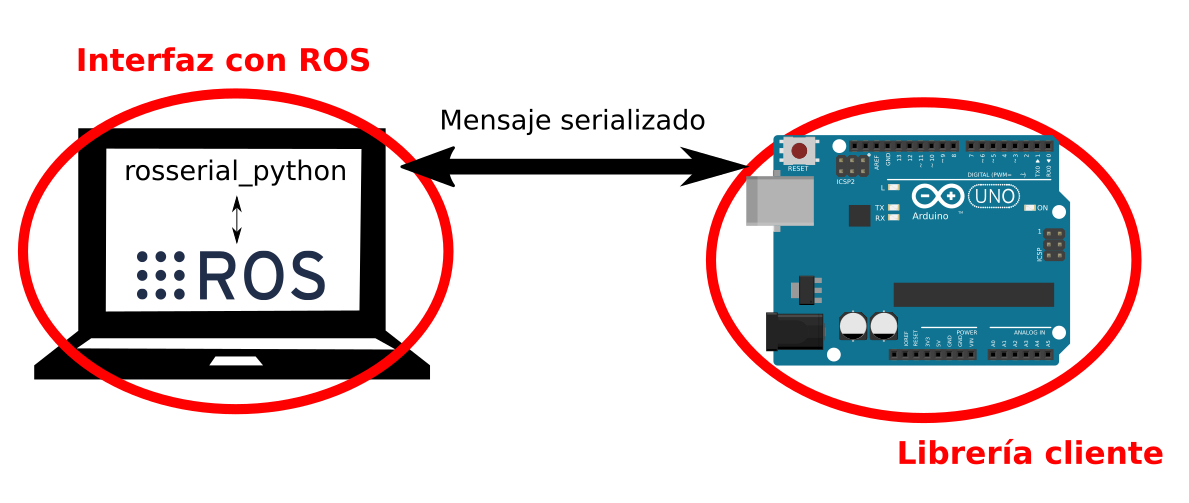
\includegraphics[scale=0.6]{./Figures/rosserial.png}
    \caption{Interacción entre ROS y rosserial que se ejecutan en un microcontrolador.}
    \label{fig:rosserial}
\end{figure}

\subsection{Transformación de coordenadas con TF}

Dentro del campo de la robótica resulta indispensable trabajar con múltiples sistemas de referencia tanto dentro del mismo robot (a la hora de representar el estado de sus articulaciones) así como para representar su estado en su universo de acción o mundo, como puede ser un mapa. Con la finalidad de y simplificar este tipo de cálculos ROS incorpora el paquete llamado TF.

Esta biblioteca fue diseñada para proveer una manera estándar para mantener el registro de los \textit{coordinate frames} o marcos de coordenadas y de realizar las transformaciones entre si mismas en todo el robot, de modo a que los usuarios puedan consumir la información de manera ordenada y sin la necesidad de ocuparse de generar las transformaciones en forma manual \citep{PAPER:3}.

TF puede operar de forma transparente en sistemas distribuidos, muy típicos en el entorno ROS. Esto significa que toda la información sobre los marcos de coordenadas de un robot se encuentran disponibles para todos los componentes de un sistema ROS en cualquiera de las computadoras que componen el sistema.

En la figura \ref{fig:tf} se visualiza un robot con múltiples articulaciones. Dado que la pose de estas se encuentra sujeta a cambios en el tiempo, también así lo hacen sus transformaciones. Por este motivo TF se encarga de monitorearlas en todo momento, lo que provee al robot la capacidad de responderse preguntas como las siguientes:

\begin{itemize}
    \item ¿a dónde se encontraba el \textit{frame} ``cabeza'' con respecto al \textit{frame} ``mundo'' hace cinco segundos?
    \item ¿cuál es la pose del objeto sostenido en mi \textit{gripper} con respecto a mi base?
    \item ¿cuál es la pose actual del \textit{frame} ``base'' en el \textit{frame} ``mapa''?
\end{itemize}


\begin{figure}[ht]
    \centering
    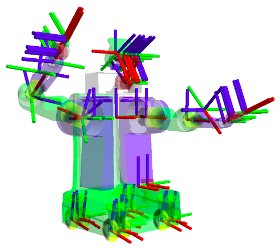
\includegraphics[scale=0.8]{./Figures/tf.png}
    \caption{Ejemplo de los \textit{frames} registrados con TF en el robot PR2, de la compañía Willow Garage.\protect\footnotemark}
    \label{fig:tf}
\end{figure}

\footnotetext{Imagen tomada de \url{http://wiki.ros.org/tf?action=AttachFile&do=get&target=frames2.png}}

\subsection{Paquete de localización robot\_localization}\label{sec:robotLocalization}

El paquete robot\_localization es una colección de estimadores no lineales para robots en espacios 2D y 3D, aunque para el aclance de este trabajo solo se hace hincapié en entornos en dos dimensiones.

Cada uno de estos estimadores permite fusionar un número arbitrario de sensores (IMUs, fuentes de odometría, sistemas de localización interna, receptores GPS, etc.) a su salida genera un vector de 15 dimensiones con el estado del robot ($x$, $y$, $z$, $roll$, $pitch$, $yaw$, $\dot{x}$, $\dot{y}$, $\dot{z}$, $\dot{roll}$, $\dot{pitch}$, $\dot{yaw}$, $\ddot{x}$, $\ddot{y}$, $\ddot{z}$).

Todos los estimadores de estados controlados por este paquete aceptan mediciones provenientes de cualquier sensor de pose siempre y cuando los mismos publiquen en alguno de los tres tipos de mensaje compatibles que se citan a continuación:

\begin{itemize}
    \item \textbf{nav\_msgs/Odometry}: posición y orientación, y velocidades lineal y angular.
    \item \textbf{sensor\_msgs/Imu}: orientación, velocidad angular y aceleración lineal.
    \item \textbf{geometry\_msgs/PoseWithCovarianceStamped}: posición y orientación.
    \item \textbf{geometry\_msgs/TwistWithCovarianceStamped}: velocidad lineal y angular.
\end{itemize}

Para este trabajo se hace uso de los dos primeros tipos de mensajes citados en la lista.

En base a estas mediciones, los estimadores publican los valores de estado filtrados de posición, orientación y velocidades lineal y angular mediante un mensaje del tipo \file{nav\_msgs/Odometry} y opcionalmente, valores de aceleración (no utilizadas en el presente trabajo).

El sotware permite a los usuarios decidir cuál de los campos de información proveidos por los sensores van a ser tomados en cuenta para la fusión en el estimador. Por este motivo, como parte de la configuración del paquete es necesario definir una matriz de booleanos para cada una de las fuentes de información o sensores para informar al estimador cuáles son los campos a tener en cuenta. A continuación se muestra la matrix completa de variables requerida para la configuración de cada una de las fuentes:

\[
    \begin{bmatrix}
        x          & y           & z         \\
        roll       & pitch       & yaw       \\
        \dot{x}    & \dot{y}     & \dot{z}   \\
        \dot{roll} & \dot{pitch} & \dot{yaw} \\
        \ddot{x}   & \ddot{y}    & \ddot{z}
    \end{bmatrix}
\]


\subsection{Paquete de navegación ros\_navigation\_stack}\label{sec:rosNavigation}

El paquete de navegación de ROS, usualmente referido como \textit{navigation stack}, es un set de algoritmos que hace uso de los sensores y las fuentes de odometría disponibles para controlar al robot es decir, le permiten moverse de un punto conocido a otro del mapa a la vez que mantiene una estimación de su posición en el espacio a cada instante.

Para que un robot pueda hacer uso de este paquete correctamente, es necesario que se satisfaga una serie de requisitos:
\begin{itemize}
    \item Solo puede utilizarse en robots con ruedas en configuración de tracción diferencial u holonómica. Cabe mencionar que el robot presentado en este trabajo es de configuración diferencial.
    \item Es necesario que el robot publique la información sobre las relaciones entre las posiciones de todas las articulaciones y sensores que lo componen.
    \item El robot deberá reportar sus velocidades lineal y angular utilizando un mensaje estándar de ROS.
    \item Un sensor del tipo LIDaR 2D deberá estar presente en el robot para generar el mapa y para el proceso de localización. Alternativamente, es posible utilizar otros tipos de sensores como cámaras de profundidad o \textit{depth cameras} o SONAR, siempre y cuando la información recolectada se publique con el tipo de mensaje adecuado.
\end{itemize}

En la figura \ref{fig:navigationStack} se puede apreciar cómo se encuentra organizado el paquete de navegación, el que utiliza dos mapas de obstáculos, uno local y otro global, que son construidos a partir de la información generada por el escáner láser en conjunto con el sistema de navegación. El mapa global es más extenso en dimiensiones que el local y está diseñado para el cálculo de trayectorias globales. Por otro lado, el mapa local es usualmente más acotado pero con mayor detalle y su objetivo es el de evadir obstáculos cercanos.

\begin{figure}[ht]
    \centering
    \def\svgwidth{350pt}
    \input{./Figures/navigation_stack.pdf_tex}
    \caption{Configuración típica del paquete de navegación en ROS.}
    \label{fig:navigationStack}
\end{figure}

Los mapas global y local son utilizados por los planeadores global y local, respectivamente. El planeador global se encarga de generar un plan para ir de un punto a otro del mapa homónimo. Por otro lado, el local se encarga de controlar los distintos actuadores del robot, por ejemplo las ruedas, para llevar a cabo el plan global pero a la vez que esquiva los obstáculos cercanos que puedan aparecer, incluso si los mismos no se encontrasen registrados en el mapa global. Esto resulta especialmente útil a la hora de esquivar obstáculos nuevos, hasta el momento desconocidos.

\section{Conceptos de robótica móvil}

En esta sección se introduce a algunos conceptos de robótica móvil que resultan de especial importancia para la comprensión en detalle del trabajo expuesto en los siguientes capítulos.

\subsection{Cinemática de un robot de tracción diferencial}

Este tipo de tracción se caracteriza por disponer de dos ruedas situadas sobre el mismo eje horizontal con la particularidad de poder ser comandadas individualmente, es decir, el sentido y velocidad de giro de cada una es independiente de la otra.

Las ventajas de este tipo de movimiento que lo hacen especialmente útil para aplicaciones como las del presente trabajo son las siguientes:

\begin{itemize}
    \item Los cálculos matemáticos requeridos para describirlo son sencillos de calcular y en consecuencia, de aplicar.
    \item Hace posible realizar giros de 360 grados alrededor del eje vertical.
    \item Es la opción elegida por los fabricantes para bases móviles comerciales de bajo costo, como el Roomba 500 descripto en la sección \ref{sec:roomba}.
\end{itemize}

\begin{figure}[ht]
    \centering
    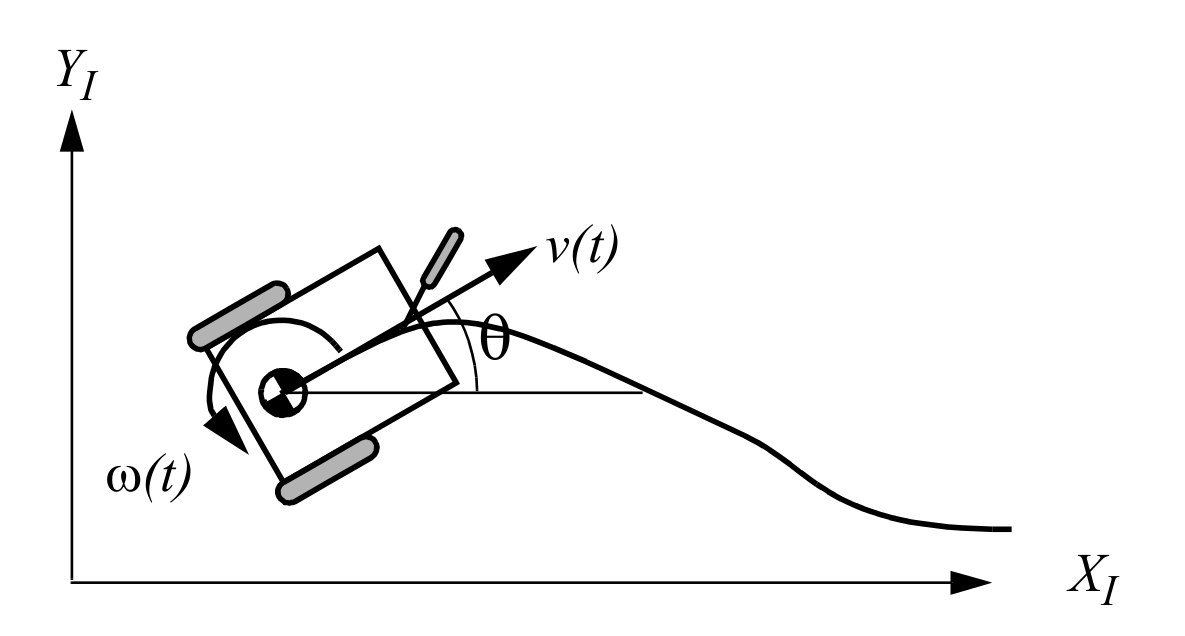
\includegraphics[scale=0.8]{./Figures/diff_drive.png}
    \caption{Descripción de la trayectoria de un robot de tracción diferencial con rueda ``loca'' o \textit{caster}.}
    \label{fig:diffdrive}
\end{figure}

Como se muestra en la figura \ref{fig:diffdrive}, es posible controlar la trayectoria descripta por el robot en un plano $(X,Y)$ mediante la manipulación de las velocidad lineal $v$ y angular $w$ del conjunto \citep{BOOK:3}. En un sistema de tracción diferencial, las fórmulas que describen la velocidad lineal $v$ y angular $w$ se muestran en la ecuacion \ref{eq:diffDriveLinear} y \ref{eq:diffDriveAngular}, respectivamente.

\begin{equation}
    \label{eq:diffDriveLinear}
    v = \frac{1}{2} \frac{V_i + V_d}{V_i - V_d}
\end{equation}

\begin{equation}
    \label{eq:diffDriveAngular}
    w = \frac{V_i - V_d}{l}
\end{equation}

donde $V_i$ y $V_d$ representan las velocidades de desplazamiento lineal de las ruedas izquierda y derecha, respectivamente y $l$ es la distancia entre ambas ruedas sobre el eje de giro.

Se generan tres casos particulares dignos de mención:
\begin{itemize}
    \item Si $V_i = V_d$, se tendrá un movimiento lineal en línea recta por lo que la velocidad angular $w$ será nula.
    \item Si $V_i = - V_d$, entonces solo habrá velocidad angular $w$ y la velocidad lineal $v$ del conjunto será nula.
    \item Si $V_i = 0$, entonces se tendrá una rotación en sentido anti-horario alrededor de la rueda izquierda con un radio de giro $l$. Se verá el mismo efecto para $V_d = 0$, esta vez con rotación en sentido horario.
\end{itemize}

\subsection{Odometría basada en encoders}

La odometría es el estudio de la estimación de la posición de robots con ruedas durante la navegación, para la que se utiliza información sobre la rotación de las ruedas que permiten estimar cambios en la posición de la base móvil en el tiempo, como se muestra en la figura \ref{fig:navigation}.

Este modelo supone que el desplazamiento de las ruedas es traducible al desplazamiento real del robot. Sin embargo, en la práctica esto no es necesariamente cierto debido a la presencia de distintos tipos de errores tales como ruedas desiguales, medidas inexactas o el resbalamiento de las ruedas en la superficie \citep{PAPER:2}. Estos motivos son los causantes de un error acumulativo no acotado que hacen que este método solo resulte apto para estimaciones en intérvalos de distancia pequeños.

Resulta necesario enriquecer esta estimación mediante su fusión con otras fuentes de información diferentes, tales como las que proveen las unidades de medición inercial, odometría visual mediante cámaras, sensores de profundidad, etc a modo de obtener una estimación final mas precisa. En este trabajo se aborda el proceso de fusión de varios de los sensores mencionados, y permite además, agregar otras fuentes de información con relativa facilidad.

\begin{figure}[ht]
    \centering
    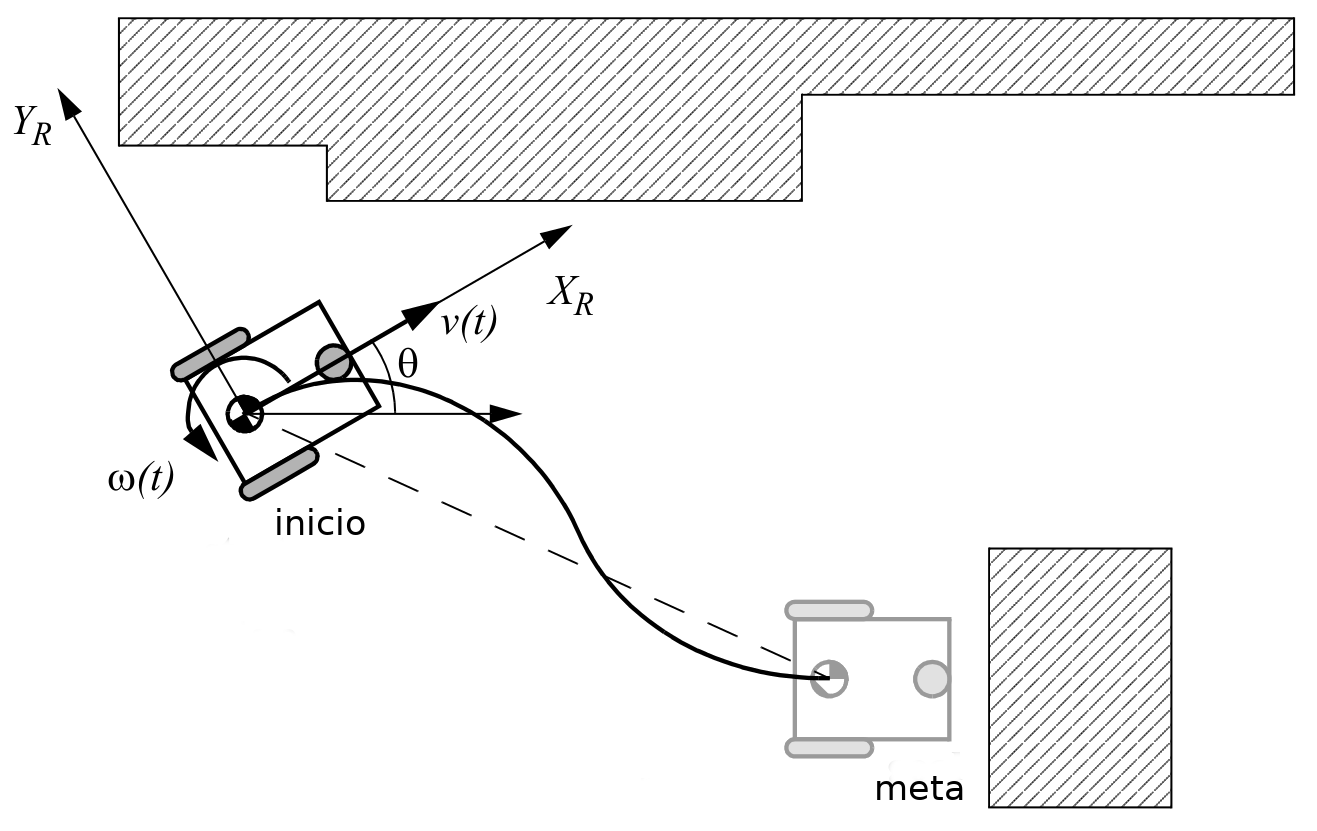
\includegraphics[scale=0.8]{./Figures/navigation.png}
    \caption{Trayectoria real descripta por un robot de tracción diferencial.}
    \label{fig:navigation}
\end{figure}

\section{iRobot Roomba 500}\label{sec:roomba}

El Roomba es un robot de limpieza fabricado y comercializado por la compañía iRobot. El primer modelo salió al mercado en el año 2002 y ha recibido siete actualizaciones desde entonces. En cada iteración, se han mejorado aspectos tanto de diseño como funcionalidad y esto le ha permitido mantenerse como el robot de limpieza con más unidades vendidas en el mundo.

Todos los Roomba incluyen una serie de sensores táctiles, ópticos y acústicos que le permiten detectar obstáculos, residuos, así como escalones o desniveles en el piso.

A nivel de locomoción, se catalogan como robots móviles con ruedas y utilizan el tipo de tracción diferencial, que consiste en dos ruedas motrices independientes que le permiten ejecutar giros de 360 grados. Esto es posible sin que el robot deba incurrir en desplazamiento lineal alguno como en el caso de los automóviles, por ejemplo.

La base móvil utilizada para este trabajo consiste en un Roomba de la serie 500 como el mostrado en la figura \ref{fig:roomba}, que fue introducido al mercado en el año 2007 y se comercializó hasta el 2017. Actualmente es posible conseguir estos equipos en condicion de usado o remanufacturado a precios muy accesibles comparado al precio de un equipo más actual.

\begin{figure}[ht]
    \centering
    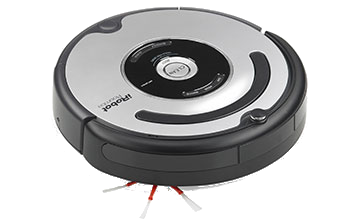
\includegraphics[scale=2.5]{./Figures/roomba.png}
    \caption{iRobot Roomba 500, utilizado como base móvil para este trabajo.\protect\footnotemark}
    \label{fig:roomba}
\end{figure}

\footnotetext{Imagen tomada de \url{https://uncrate.com/assets_c/2009/04/roomba-560-stretched-thumb-960x640-3177.jpg}}

\subsection{Roomba Open Interface}\label{sec:openInterface}
Todos los Roomba lanzados a partir del año 2005 son compatibles con una interfaz de comunicación serial denominada Roomba Open Interface, a la que es posible acceder mediante la conexión a un puerto físico disponible en la placa madre del robot. Esto habilita al usuario a todo tipo de interacción con el hardware del robot, como consultar la lectura de cada uno de sus sensores o comandar sus actuadores. Este protocolo ha sido actualizado a la par de las sucesivas actualizaciones del Roomba para ofrecer nuevas funcionalidades o mejoras y en cada caso, se encuentra acompañado de un documento oficial por parte de iRobot en formato PDF\protect\footnotemark.

\footnotetext{Imagen tomada de \url{https://cdn-shop.adafruit.com/datasheets/create_2_Open_Interface_Spec.pdf}}


\subsection{Conexionado del robot por puerto serie}

En la figura \ref{fig:roombaPinout} y la tabla \ref{tab:Pines} se exponen respectivamente, la distribución de pines en el conector y su conexión correspondiente para entablar comunicación con el robot mediante el puerto Mini-DIN.

\begin{figure}[ht]
    \centering
    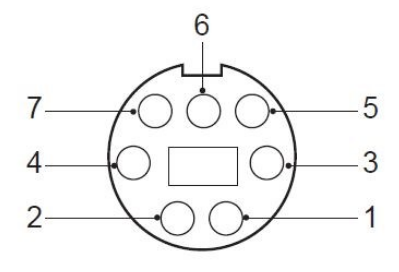
\includegraphics[scale=.4]{./Figures/pinout.png}
    \caption{Distribución de pines en el conector hembra Mini-DIN.}
    \label{fig:roombaPinout}
\end{figure}

\begin{table}[h]
    \centering
    \caption{Referencia de pines en conector Mini-DIN hembra.}
    \label{tab:Pines}
    \begin{tabular}{rll}
        \toprule
        \multicolumn{1}{l}{Pin} & Nombre & Descripción                                  \\
        \midrule
        1                       & Vpwr   & Positivo directo de la batería (no regulado) \\
        2                       & Vpwr   & Positivo directo de la batería (no regulado) \\
        3                       & RXD    & 0 - 5 VCC Entrada serie                      \\
        4                       & TXD    & 0 - 5 VCC Salida serie                       \\
        5                       & BRC    & Cambio de \textit{baud-rate}                 \\
        6                       & GND    & Tierra del robot                             \\
        7                       & GND    & Tierra del robot                             \\
        \bottomrule
    \end{tabular}
\end{table}

\section{Placa de desarrollo STM32-NUCLEO}

Es una familia de placas de desarrollo elaboradas por la compañía ST. Entre sus características principales se destacan:

\begin{itemize}
    \item Bajo costo
    \item Compatibilidad con \textit{shields} de Arduino
    \item Programador/debugger ST-Link integrado
    \item biblioteca del tipo HAL con variados ejemplos de código
\end{itemize}

Con el fin de garantizar la escalabilidad del sistema, para este proyecto se optó por una de las placas mas avanzadas de esta familia, denominada NUCLEO-F746ZG y mostrada en la figura \ref{fig:stm32nucleo}. Esta provee un microcontrolador ARM Cortex-M7 con FPU de doble precisión, 320 kB de RAM, así como 1 MB de Flash. Ofrece además conexión Ethernet y una amplia cantidad de GPIOs.

\begin{figure}[ht]
    \centering
    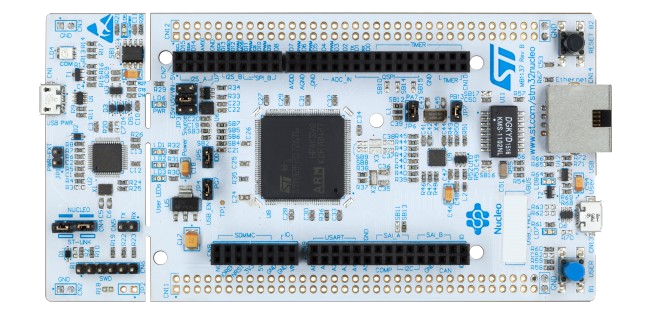
\includegraphics[scale=1.5]{./Figures/stm32nucleo.png}
    \caption{Placa de desarrollo STM32 NUCLEO-F746ZG elegida para comandar el robot.\protect\footnotemark}
    \label{fig:stm32nucleo}
\end{figure}

\footnotetext{Imagen tomada de \url{https://www.carminenoviello.com/wp-content/uploads/2015/12/nucleo_144_large-2-660x330.jpg}}

\section{Sensor Kinect 360}

El Kinect para Xbox 360 o simplemente Kinect, es un dispositivo de captura de movimiento diseñado por la empresa Microsoft que utiliza tecnología desarrollada por la empresa israelita PrimeSense.

Cuenta con una cámara que captura imágenes en formato RGB, un \textit{array} de micrófonos, así como un sensor de profundidad. Si bien existen otras características extra que podrían mencionarse, vale la pena detenerse en esta última y explicar en qué consiste, puesto que se la utilizó de manera extensiva en el trabajo propuesto para la generación de mapas del robot.

\subsection{Imagen de profundidad}

El sensor de profundidad del Kinect consiste en un proyector de nube de puntos infrarrojos combinado con un sensor CMOS monocromático, similar al de una cámara fotográfica. Funcionando en combinación, estos dos elementos son capaces de captar la información necesaria para que un ASIC genere con ella una imagen de profundidad o \textit{Depth map}, que consiste en un mapa de bits con información sobre la distancia relativa entre el sensor y los objetos detectados. En la figura \ref{fig:depthMap} se puede apreciar una imagen de profundidad generada mediante el sensor Kinect en el que se distingue claramente la silueta de una persona en un entorno con diferentes objetos. Las distintas tonalidades de grises visualizadas son una representación de la distancia del objeto al sensor, por lo que para objetos cercanos veremos píxeles de color gris mas claro mientras que para objetos lejanos se verán mas oscuros.

\begin{figure}[ht]
    \centering
    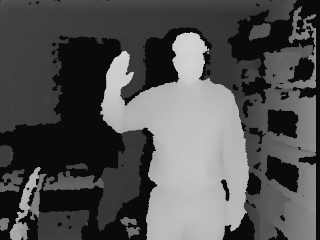
\includegraphics[scale=2.0]{./Figures/depth_map.png}
    \caption{\textit{Depth map} de la silueta de una persona.}
    \label{fig:depthMap}
\end{figure}

\section{Unidad de medición inercial}

Una unidad de medición inercial o IMU por sus siglas en inglés, es un dispositivo electrónico capaz de medir y reportar la velocidad angular y en algunos casos, el campo magnético que rodea al cuerpo.

Las IMU funcionan detectando la aceleración lineal mediante uno o más acelerómetros y la tasa de rotación usando uno o más giroscopios. Algunos de estos dispositivos incluyen también un magnetómetro que se utiliza comúnmente como una referencia de rumbo.

Las configuraciones típicas de una IMU continenen un acelerómetro, un giroscopio y un magnetómetro para cada uno de los tres ejes de giros y fuerzas del vehículo: cabeceo, alabeo y guiñada, que se muestran en la figura ref{fig:imu}. Para el caso particular del robot móvil propuesto en este trabajo, solo se hace uso de las aceleraciones: angular en el eje Z y lineal en el eje X, respectivamente.

\begin{figure}[ht]
    \centering
    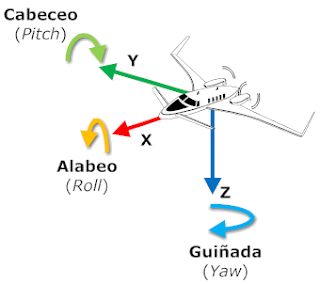
\includegraphics[scale=1.5]{./Figures/imu.png}
    \caption{Ejes de giros y fuerzas de un vehículo.\protect\footnotemark}
    \label{fig:depthMap}
\end{figure}

\footnotetext{Imagen tomada de \url{http://skiras.blogspot.com/2012/10/4copter-conceptos-i-ejes-giros-y-fuerzas.html}}

\subsection{Sensor MPU6050}\label{sec:mpu6050}

El dispositivo MPU-6050 mostrado en la figura \ref{fig:mpu6050} combina en el mismo chip un giroscopio de 3 ejes con un acelerómetro también de 3 ejes. Mediante lo que el fabricante denomina \textit{Digital Motion Processor} o DMP, esta IMU es capaz de procesar algoritmos de fusión de datos de 6 ejes, usualmente ejecutados en un microcontrolador o DSP mediante un filtro de Kalman o similar. Si bien el chip no incluye un magnetómetro, sí ofrece una interfaz I2C que posibilita conectarla a un magnetómetro externo, de este modo el DMP puede aprovechar la información de campo magnético en en sus algoritmos de fusión para generar resultados más precisos.

\begin{figure}[ht]
    \centering
    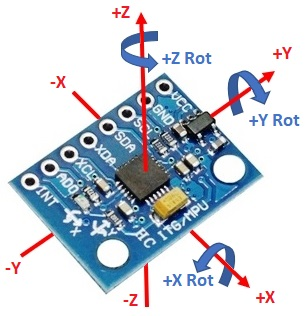
\includegraphics[scale=0.45]{./Figures/mpu6050.jpg}
    \caption{Sensor MPU-6050 con sus ejes de giros y fuerzas.}
    \label{fig:mpu6050}
\end{figure} 
% !TeX root = ./../memoria.tex
\chapter{Diseño e Implementación} % Main chapter title

\label{Chapter3} % Change X to a consecutive number; for referencing this chapter elsewhere, use \ref{ChapterX}

\definecolor{mygreen}{rgb}{0,0.6,0}
\definecolor{mygray}{rgb}{0.5,0.5,0.5}
\definecolor{mymauve}{rgb}{0.58,0,0.82}

%%%%%%%%%%%%%%%%%%%%%%%%%%%%%%%%%%%%%%%%%%%%%%%%%%%%%%%%%%%%%%%%%%%%%%%%%%%%%
% parámetros para configurar el formato del código en los entornos lstlisting
%%%%%%%%%%%%%%%%%%%%%%%%%%%%%%%%%%%%%%%%%%%%%%%%%%%%%%%%%%%%%%%%%%%%%%%%%%%%%
\lstset{ %
  backgroundcolor=\color{white},   % choose the background color; you must add \usepackage{color} or \usepackage{xcolor}
  basicstyle=\footnotesize,        % the size of the fonts that are used for the code
  breakatwhitespace=false,         % sets if automatic breaks should only happen at whitespace
  breaklines=true,                 % sets automatic line breaking
  captionpos=b,                    % sets the caption-position to bottom
  commentstyle=\color{mygreen},    % comment style
  deletekeywords={...},            % if you want to delete keywords from the given language
  %escapeinside={\%*}{*)},          % if you want to add LaTeX within your code
  %extendedchars=true,              % lets you use non-ASCII characters; for 8-bits encodings only, does not work with UTF-8
  %frame=single,	                % adds a frame around the code
  keepspaces=true,                 % keeps spaces in text, useful for keeping indentation of code (possibly needs columns=flexible)
  keywordstyle=\color{blue},       % keyword style
  language=[ANSI]C,                % the language of the code
  %otherkeywords={*,...},           % if you want to add more keywords to the set
  numbers=left,                    % where to put the line-numbers; possible values are (none, left, right)
  numbersep=5pt,                   % how far the line-numbers are from the code
  numberstyle=\tiny\color{mygray}, % the style that is used for the line-numbers
  rulecolor=\color{black},         % if not set, the frame-color may be changed on line-breaks within not-black text (e.g. comments (green here))
  showspaces=false,                % show spaces everywhere adding particular underscores; it overrides 'showstringspaces'
  showstringspaces=false,          % underline spaces within strings only
  showtabs=false,                  % show tabs within strings adding particular underscores
  stepnumber=1,                    % the step between two line-numbers. If it's 1, each line will be numbered
  stringstyle=\color{mymauve},     % string literal style
  tabsize=2,	                   % sets default tabsize to 2 spaces
  title=\lstname,                  % show the filename of files included with \lstinputlisting; also try caption instead of title
  morecomment=[s]{/*}{*/}
}


%----------------------------------------------------------------------------------------
%	SECTION 1
%----------------------------------------------------------------------------------------
\section{Análisis del software}
 
La idea de esta sección es resaltar los problemas encontrados, los criterios utilizados y la justificación de las decisiones que se hayan tomado.

Se puede agregar código o pseudocódigo dentro de un entorno lstlisting con el siguiente código:

\begin{verbatim}
\begin{lstlisting}[caption= "un epígrafe descriptivo"]
	las líneas de código irían aquí...
\end{lstlisting}
\end{verbatim}

A modo de ejemplo:

\begin{lstlisting}[label=cod:vControl,caption=Pseudocódigo del lazo principal de control.]  % Start your code-block

#define MAX_SENSOR_NUMBER 3
#define MAX_ALARM_NUMBER  6
#define MAX_ACTUATOR_NUMBER 6

uint32_t sensorValue[MAX_SENSOR_NUMBER];		
FunctionalState alarmControl[MAX_ALARM_NUMBER];	//ENABLE or DISABLE
state_t alarmState[MAX_ALARM_NUMBER];						//ON or OFF
state_t actuatorState[MAX_ACTUATOR_NUMBER];			//ON or OFF

void vControl() {

	initGlobalVariables();
	
	period = 500 ms;
		
	while(1) {

		ticks = xTaskGetTickCount();
		
		updateSensors();
		
		updateAlarms();
		
		controlActuators();
		
		vTaskDelayUntil(&ticks, period);
	}
}
\end{lstlisting}




%% !TeX root = ./../memoria.tex
% Chapter Template

\chapter{Experimentos y resultados} % Main chapter title

\label{Capitulo4}

En este capítulo se detallan las pruebas que fueron realizadas sobre los distintos módulos de hardware y software que componen al robot así como los resultados de las pruebas de campo que se llevaron a cabo.

\section{Pruebas unitarias en el robot}
que le siguieron
En esta sección se describen las pruebas funcionales ejecutadas sobre cada uno de los módulos que componen el robot de manera aislada. Esto permitió encontrar problemas puntuales y reducir las fuentes de error para las pruebas de integración que le siguieron.

\subsection{Validación de conexión bidireccional Roomba-microcontrolador}

Descripción del setup del microcontrolador usando 2 conexiones UART simultáneas.

Envío de comandos de: conexión, desconexión.

\begin{figure}[ht]
    \centering
    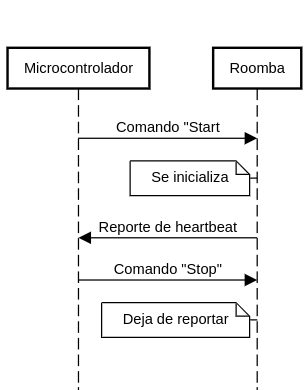
\includegraphics[scale=0.6]{./Figures/comm_test2.png}
    \caption{Diagrama de secuencias ejecutadas durante el test de comunicación entre el microcontrolador y el Roomba.}
    \label{fig:secMicroRoomba}
\end{figure}

\subsection{Validación de conexión bidireccional microcontrolador-ROS}

Descripción de la conexión con ROS usando un mensaje de ``ping'' con una doble confirmación. En el diagrama de la figura \ref{fig:secMicroROS} se muestra la secuencia de acciones llevadas a cabo para la prueba.

\begin{figure}[ht]
    \centering
    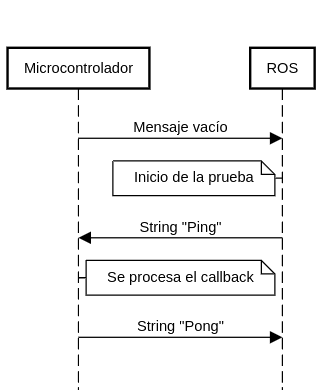
\includegraphics[scale=0.6]{./Figures/comm_test1.png}
    \caption{Diagrama de secuencias ejecutadas durante el test entre el microcontrolador y una PC con ROS.}
    \label{fig:secMicroROS}
\end{figure}

\subsection{Validación de frenado de emergencia}

El Roomba funciona de una manera tal que si recibe un comando de velocidad, este se aplica al robot por tiempo indefinido. Con el fin de prevenir riesgos, se implementó en el controlador un sistema de frenado de emergencia que responde a los siguientes pasos:

\begin{itemize}
    \item Se activa en cuanto se recibe un comando de velocidad distinto de cero.
    \item Se activa una tarea periódica, ejecutada cada 500 ms en donde se comprueba la existencia de al menos un mensaje nuevo en el tópico /cmd\_vel.
    \item En caso que no haya ningún mensaje, la tarea envía la orden de detener el robot.
\end{itemize}

\subsection{Validación de desplazamiento efectivo del robot}

El Roomba implementa su propio sistema de control interno a lazo cerrado de los motores para llevar sus ruedas hasta el \textit{set point} requerido por los comandos de velocidad. En vista de que esta funcionalidad resulta crítica para el sistema, se desarrolló un caso de prueba especial para velocidades tanto positivas como negativas que se describe a continuación:

\begin{itemize}
    \item mediante un script de Python conectado a ROS se envió un comando que establece la velocidad de ambas ruedas a 0,1 m/s por una duración de 10 s es decir, el equivalente a un desplazamiento lineal de 1 m.
    \item mediante una cinta métrica se compararon los valores esperados con el desplazamiento lineal real.
\end{itemize}

Un análisis cualitativo de los resultados expuestos en la tabla \ref{tab:desplazamientoRobot} evidencia que el sistema de control de velocidades interno del Roomba asume que la masa del robot es constante y no toma en cuenta el peso del hardware agregado. Como consecuencia los comandos para mover el robot muestran un porcentaje de error importante.

\begin{table}[!htbp]
    \centering
    \caption[Desplazamiento robot]{Resultados de validación de desplazamiento efectivo del robot}
    \begin{tabular}{lccc}
        \toprule
        \textbf{Movimiento} & \textbf{Desplazamiento} & \textbf{Desplazamiento} & \textbf{Error}    \\
                            & \textbf{esperado}       & \textbf{obtenido}       & \textbf{obtenido} \\
        \midrule
        Lineal positivo 1 m & 1,0 m                   & 0,98 m                  & 2 \%              \\
        Lineal negativo 1 m & -1,0 m                  & -0,96 m                 & 4 \%              \\
        \bottomrule
        \hline
    \end{tabular}
    \label{tab:desplazamientoRobot}
\end{table}

Como medida paliativa se decidió no utilizar el robot en modo reversa para las tareas de mapeo de manera a reducir el error acumulativo. Vale mencionar que dejando de depender del control de velocidad interno del Roomba e implementando un sistema de control externo al mismo en el microcontrolador, permitiría solucionar este error. Esta posibilidad se menciona en las conclusiones como uno de los siguientes pasos.

\subsection{Validación de lectura de encoders}

Dado que es posible obtener las lecturas crudas de los encoders del robot, se realizó la comprobación siguiente de manera similar a la prueba anterior:

\begin{itemize}
    \item mediante un script de Python conectado a ROS se envió un comando de velocidad que establece la velocidad de ambas ruedas a 0.1 m/s por una duración de 10 s es decir, el equivalente a un desplazamiento de 1 m.
    \item mediante los encoders se obtuvo la cantidad de \textit{ticks} o cuentas ocurridas durante dicho periodo.
    \item se calculó el desplazamiento estimado mediante la siguiente fórmula obtenida a partir del documento de especificaciones del fabricante \citep{PAPER:5}:
          \begin{equation}
              Disancia = nTicks / 4498,9125
          \end{equation}

\end{itemize}

Los resultados expuestos en la tabla \ref{tab:lecturaEncoders} muestran ciertas similitudes con los resultados de la prueba anterior en el sentido que el robot reporta un movimiento más ``corto'' que el que le fue comandado. Dado que el número de \textit{ticks} de la rueda izquierda es mayor que el de la derecha, es correcto asumir que el robot describió un movimiento curvilíneo con radio de giro hacia la derecha, lo que pudo comprobarse por el autor al observar la posición del robot al final de la prueba.

\begin{table}[!htbp]
    \centering
    \caption[Lectura de encoders]{Resultados de validación de lectura de encoders}
    \begin{tabular}{lcccccc}
        \toprule
        \multirow{2}{*}{\textbf{Movimiento}} & \multicolumn{2}{l}{\textbf{Ticks esperados}} & \multicolumn{2}{l}{\textbf{Ticks obtenidos}} & \multicolumn{2}{l}{\textbf{Error obtenido}}                                                 \\
                                             & \textbf{Izq.}                                & \textbf{Der.}                                & \textbf{Izq.}                               & \textbf{Der.} & \textbf{Izq.} & \textbf{Der.} \\
        \midrule
        Lineal positivo 1 m                  & 2250                                         & 2250                                         & 2201                                        & 2137          & 2,22 \%       & 5,28 \%       \\
        Lineal negativo 1 m                  & 2250                                         & 2250                                         & 2194                                        & 2103          & 2,55 \%       & 6,99 \%       \\
        \bottomrule
        \hline
    \end{tabular}
    \label{tab:lecturaEncoders}
\end{table}

\subsection{Validación de lecturas crudas de la IMU}

Esta prueba consistió en graficar las lecturas de las seis variables registradas por el sensor durante una secuencia de tres movimientos a la que fue sometido.

Para esta prueba se partió de un estado inicial con la IMU quieta, con el plano definido por sus ejes $(X,Y)$ en posición normal al vector de aceleración de la gravedad (que apunta al centro de la Tierra). Para todas las pruebas se utilizó la convención ``North-East-Down'' \protect\footnotemark que el sensor adopta por defecto.

\footnotetext{Coordenadas locales del plano tangente NED: \url{https://en.wikipedia.org/wiki/Local\_tangent\_plane\_coordinates}}

Basado en las lecturas del acelerómetro de la figura \ref{fig:aceleracionLineal} se describen las observaciones realizadas:

\begin{itemize}
    \item en la primera columna se observa el vector de aceleración de la gravedad de aproximadamente 9,8 $m/s^2$ apuntando en la dirección negativa del eje $Z$.
    \item en la segunda columna se observa el mismo vector de aceleración, esta vez trasladado en dirección del eje $X$ negativo.
    \item finalemente en la tercera columna se observa al vector transladado en dirección al eje $Y$ negativo.
\end{itemize}


\begin{figure}[ht]
    \centering
    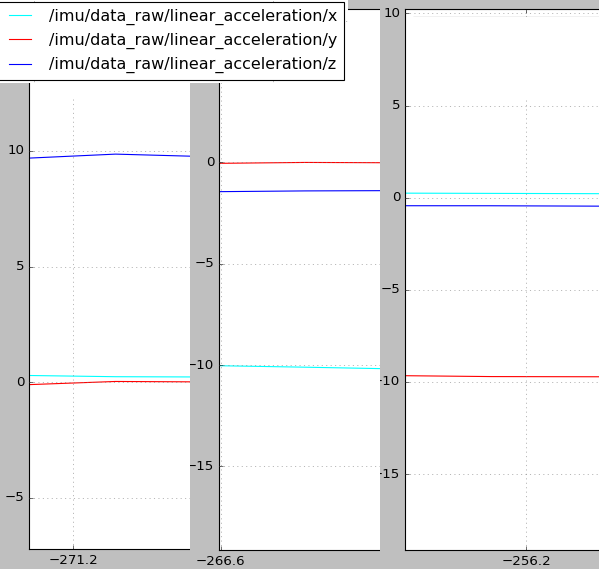
\includegraphics[scale=0.4]{./Figures/linear_acceleration.png}
    \caption{Gráfico de aceleraciones lineales sobre cada uno de los ejes registrados durante las tres posiciones de prueba.}
    \label{fig:aceleracionLineal}
\end{figure}


Para las gráficas del giroscopio se procedió con la misma metodología utilizada para el acelerómetro. La diferencia en estas pruebas radica en que los valores medidos por el giroscopio son instantáneos, ya que corresponden a velocidades angulares alrededor de los ejes durante los movimientos efectuados, y desaparecen al dejar de mover la IMU. Por este motivo se presentan seis gráficas que fueron distribuidas en las figuras \ref{fig:velocidadAngular1} y \ref{fig:velocidadAngular2} de izquierda a derecha, donde se muestran los valores adoptados por los tres ejes del giroscopio durante los movimientos descriptos a continuación:

\begin{enumerate}
    \item giro alrededor del eje $Y$ en sentido antihorario.
    \item giro alrededor del eje $Y$ en sentido horario.
    \item giro alrededor del eje $X$ en sentido antihorario.
    \item giro alrededor del eje $X$ en sentido horario.
    \item giro alrededor del eje $Z$ en sentido antihorario.
    \item giro alrededor del eje $Z$ en sentido horario.
\end{enumerate}

\begin{figure}[ht]
    \centering
    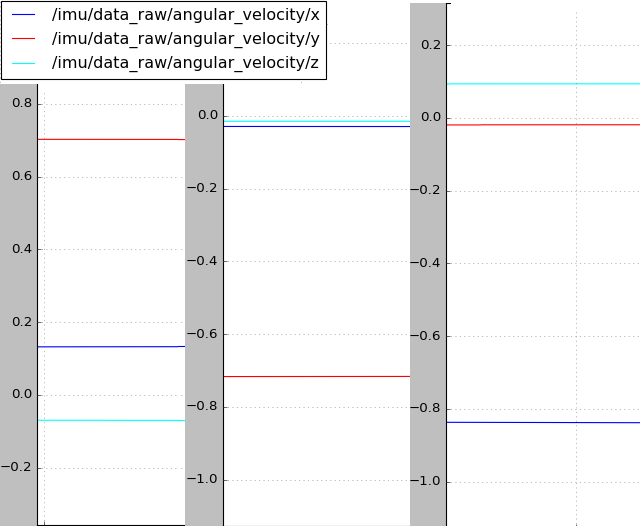
\includegraphics[scale=0.42]{./Figures/angular_velocity_1.png}
    \caption{Gráfico de velocidades angulares durante los movimientos 1, 2 y 3.}
    \label{fig:velocidadAngular1}
\end{figure}

\begin{figure}[ht]
    \centering
    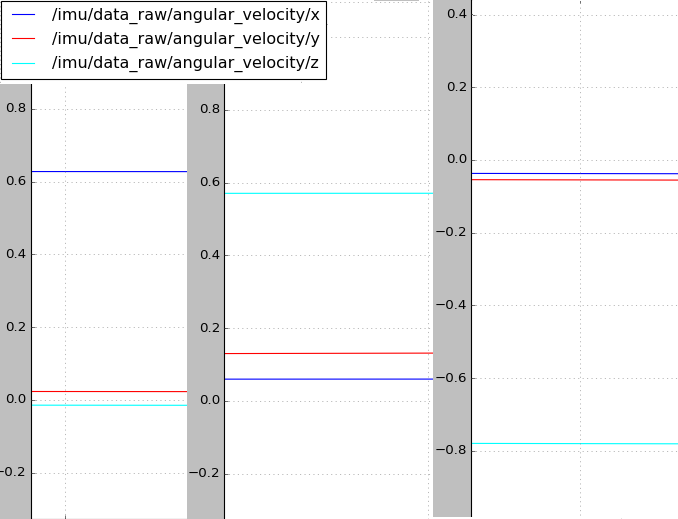
\includegraphics[scale=0.42]{./Figures/angular_velocity_2.png}
    \caption{Gráfico de velocidades angulares durante los movimientos 4, 5 y 6.}
    \label{fig:velocidadAngular2}
\end{figure}


\section{Pruebas unitarias en la PC}

En esta sección se describen las pruebas realizadas sobre los resultados arrojados por los componentes de software ejecutados en la PC. Estos se utilizan para procesar los datos crudos arrojados por los sensores y generar información en un formato aprovechable por ROS.

\subsection{Validación de cálculo de odometría con encoders}

Esta prueba tuvo como objetivo validar el correcto funcionamiento del programa lubo\_odom\_node, que consume las lecturas de encoders y realiza con estas una estimación de la posición y orientación del robot en un plano $(X,Y)$.

Para la validación de esta característica, la prueba se realizó siguiendo los siguientes pasos:
\begin{enumerate}
    \item se marcó la pose inicial del robot en el suelo.
    \item se comandaó el robot con un \textit{joystick} a una velocidad aproximada de 0,1 $m/s$.
    \item se movió el robot aproximadamente 1 $m$ hacia adelante.
    \item se hizo girar el robot aproximadamente 90 grados.
    \item se movió nuevamente el robot aproximadamente 1 $m$ hacia adelante.
    \item se midió la distancia lineal entre el punto de inicio y el punto final del robot.
    \item se obtuvieron las componentes en $X$ e $Y$ del vector de distancia trazado en el punto anterior.
    \item se comparararon estas medidas con los valores arrojados por la odometría, y con esto se calculó el error. Esta información se expone en la tabla \ref{tab:odometriaEncoders}.
\end{enumerate}

\begin{table}[!htbp]
    \centering
    \caption[Odometria de encoders]{Resultados de validación de odometría de encoders}
    \begin{tabular}{lccc}
        \toprule
        \textbf{Variable}  & \textbf{Medición esperada} & \textbf{Medición reportada} & \textbf{Error obtenido} \\
        \midrule
        Posición en $X$    & 1 m                        & 1,04 m                      & 4 \%                    \\
        Posición en $Y$    & 1 m                        & 0,8 m                       & 20 \%                   \\
        Orientación en $Z$ & -0,785 rad                 & -0,729 rad                  & 7,73 \%                 \\
        \bottomrule
        \hline
    \end{tabular}
    \label{tab:odometriaEncoders}
\end{table}

% \subsection{Validación de estimador de pose con filtro Madwick para IMU}

% El IMU MPU6050 no ofrece medición de campo magnético, por este motivo la información que provee resulta limitada e insuficiente para estimar la orientación absoluta del dispositivo.
% Existen varias soluciones diferentes distintas para esta problemática pero para este trabajo se eligió utilizar un estimador de pose, es decir, un filtro especial que toma la información en bruto de acelerómetro y giroscopio y a su salida provee además de los valores filtrados de sus entradas, una estimación de la orientación del sensor.

% Descripción de los resultados arrojados por la IMU MPU6050 en bruto. Gráfico de rqt\_plot
% Resultados arrojados por las mismas mediciones, esta vez con el filtro activado.

\subsection{Validación de estimador de odometría con encoders + IMU}

Gracias a la aplicación de un Filtro de Kalman Extendido por parte del paquete robot\_localization, fue posible fusionar la información provista por el cálculo de odometría de encoders junto con el estimador de pose de la IMU.

Este procedimiento consistió en comparar los resultados obtenidos con la prueba de odometría de encoders pura del punto anterior y la estimación de odometria resultante de combinar este valor con la pose de la IMU. El procedimiento ejecutado fue el mismo que se utilizó en el punto anterior y los resultados se exponen en la tabla \ref{tab:odometriaFusion}.

\begin{table}[!htbp]
    \centering
    \caption[Fusión de odometría con IMU]{Resultados de validación del estimador de odometría mediante la fusión de datos de encoders e IMU.}
    \begin{tabular}{lccc}
        \toprule
        \textbf{Variable}  & \textbf{Medición esperada} & \textbf{Medición reportada} & \textbf{Error obtenido} \\
        \midrule
        Posición en $X$    & 1 m                        & 1,01 m                      & 1 \%                    \\
        Posición en $Y$    & 1 m                        & 0,98 m                      & 2 \%                    \\
        Orientación en $Z$ & -0,785 rad                 & -0,786 rad                  & 0,13 \%                 \\
        \bottomrule
        \hline
    \end{tabular}
    \label{tab:odometriaFusion}
\end{table}

Gracias a que ambos tests se encargan de reproducir el mismo escenario fue posible comparar ambos resultados y obtener el porcentaje de mejora ofrecido por la fusión de datos sobre el error absoluto. Los resultados de esta comparación se pueden apreciar en la tabla \ref{tab:comparacionOdom}. Como puede observarse la mejora obtenida debido a la fusión fue muy significativa.

\begin{table}[!htbp]
    \centering
    \centering
    \caption[Comparacion de calculos de odometría]{Resultados obtenidos al comparar las lecturas arrojadas por la odometría de encoders ``pura'' y la odometría resultante de la fusión de encoders e IMU.}
    \begin{tabular}{lccc}
        \toprule
        \textbf{Variable}  & \textbf{Técnica 1} & \textbf{Técnica 2} & \textbf{Porcentaje de mejora} \\
        \midrule
        Posición en $X$    & 1,04 m             & 1,01 m             & \textasciitilde300 \%         \\
        Posición en $Y$    & 0,8 m              & 0,98 m             & \textasciitilde1000 \%        \\
        Orientación en $Z$ & -0,729 rad         & -0,786 rad         & \textasciitilde6000 \%        \\
        \bottomrule
    \end{tabular}
    \label{tab:comparacionOdom}
\end{table}


\section{Pruebas de integración en campo}

En esta sección se describen las pruebas funcionales ejecutadas sobre cada uno de los módulos que componen el robot de manera aislada. Esto permitió encontrar problemas puntuales y reducir las fuentes de error para las pruebas de integración.

\subsection{Generación de mapa con gmapping}

Esta prueba consistió en la generación de un mapa de grillas de ocupación. Este mapa consiste en una representación similar a la de un plano en dos dimensiones similar a los que se utilizan en obras civiles. Las grillas en negro representan una sección ocupada mientras que las blancas representan un área libre.


Para que el resultado obtenido a partir de este procedimiento fuera lo suficientemente preciso como para utilizarse en la tarea de localizar al robot fue necesario que la fuente de odometría fuera muy precisa, motivo por el que resultó indispensable el uso de la fuente de odometría filtrada con información de la IMU.

En las figuras \ref{fig:mapaFeo} se puede apreciar el mapa obtenido a partir de la odometría de encoders ``pura''. Este primer mapa resulta totalmente inutilizable para tareas de navegación puesto que no refleja la morfología real del recinto. Por el contrario, el mapa de la figura \ref{fig:mapaLindo} se generó utilizando la fuente de odometría filtrada con IMU. A pesar de sus restricciones, este último mapa resultó suficiente para las tareas de localización y navegación del robot.


\begin{figure}[ht]
    \centering
    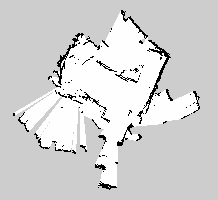
\includegraphics[scale=1.0]{./Figures/mapa_feo.png}
    \caption{Mapa obtenido utilizando odometría de encoders ``pura''.}
    \label{fig:mapaFeo}
\end{figure}

\begin{figure}[ht]
    \centering
    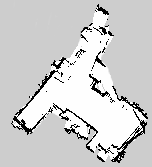
\includegraphics[scale=1.2]{./Figures/mapa_lindo.png}
    \caption{Mapa obtenido utilizando odometría filtrada.}
    \label{fig:mapaLindo}
\end{figure}


%TODO: agregar imagenes de 1) Mapa horrible sin ekf 2) mapita decente con ekf.

\subsection{Localización en mapa con amcl}

% Tal como se describió en la sección \ref{sec:amcl}, amcl es un paquete para ROS que provee al robot la capacidad de encontrar su posición y orientación de un mapa previamente provisto. Esta prueba consistió en la utilización del mapa generado de la sala de estar del departamento del autor. Este fue provisto a la herramienta amcl mediante el servidor de parámetros de ROS y luego se procedió a teleoperar el robot mediante un \textit{joystick} inalámbrico. El procedimiento utilizado fue el siguiente:
Amcl es un paquete para ROS que provee al robot la capacidad de encontrar su posición y orientación de un mapa previamente provisto. Esta prueba consistió en la utilización del mapa generado de la sala de estar del departamento del autor. Este fue provisto a la herramienta amcl mediante el servidor de parámetros de ROS y luego se procedió a teleoperar el robot mediante un \textit{joystick} inalámbrico. El procedimiento utilizado fue el siguiente:

\begin{enumerate}
    \item se colocó el robot en una pose aleatoria en el mapa como se muestra en la figura \ref{fig:sinLocalizar}.
    \item por medio del \textit{joystick} se hizo girar al robot en círculos en sentido horario hasta completar dos vueltas completas de 360 grados a una velocidad angular aproximada de 0,5 rad/s.
    \item se aplicó el mismo procedimiento para un giro en sentido anti-horario.
\end{enumerate}


\begin{figure}[ht]
    \centering
    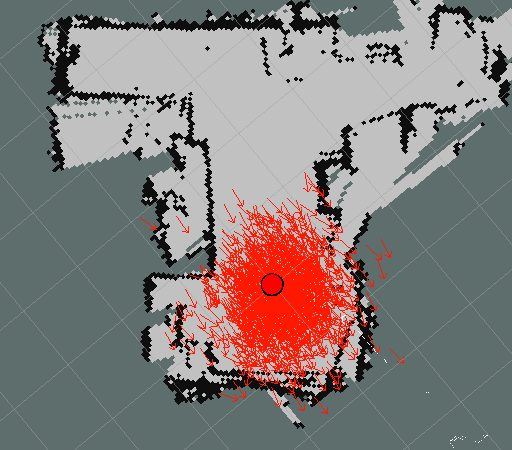
\includegraphics[scale=0.4]{./Figures/sin_localizar.png}
    \caption{Captura de pantalla de RViz con el robot aún sin localizarse. Las flechas rojas muestran las posibles poses del robot en el mapa.}
    \label{fig:sinLocalizar}
\end{figure}

El resultado final se puede apreciar en la figura \ref{fig:robotLocalizado}. En esta imagen, tanto la posición en $X$ e $Y$ del robot con respecto al mapa han sido estimadas y así también su orientación respecto al eje $Z$.

\begin{figure}[ht]
    \centering
    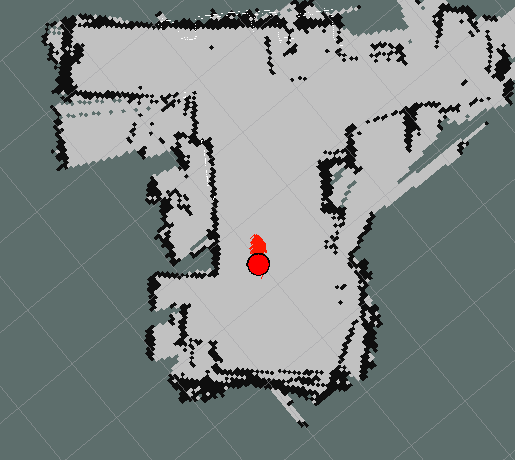
\includegraphics[scale=0.4]{./Figures/robot_localizado.png}
    \caption{Captura de pantalla de RViz con el robot localizado. En este momento las flechas rojas han convergido hacia una misma región donde se estima que se encuentra el robot.}
    \label{fig:robotLocalizado}
\end{figure}

\subsection{Navegación en mapa con move\_base}

% Así como se describe en la sección \ref{sec:move_base}, move\_base provee la funcionalidad necesaria para mover al robot dentro del mapa provisto, para lo cual la herramienta se encarga de calcular una ruta de navegación desde el punto en que el robot se encuentra al momento de enviarse la orden y otro punto cualquiera del mapa.
El paquete move\_base provee la funcionalidad necesaria para mover al robot dentro del mapa provisto, para lo cual la herramienta se encarga de calcular una ruta de navegación desde el punto en que el robot se encuentra al momento de enviarse la orden y otro punto cualquiera del mapa.

Esta prueba consistió en indicar a la herramienta que deseábamos mover el robot de un punto a otro en el mapa. Para esto fue necesario cumplir con ciertos requisitos previos:

\begin{enumerate}
    \item un mapa estático debió ser provisto al servidor de mapas de ROS.
    \item el robot debió encontrarse previamente localizado en el mapa.
\end{enumerate}

El envío de consigna se realiza mediante la herramienta RViz, que se representa mediante un vector de color verde en el mapa. Su punto de origen representa la posición deseada mientras que su dirección representa la orientación final del robot. En las figuras \ref{fig:comandoNavegación} y \ref{fig:robotEnSetpoint} se puede apreciar al robot en su punto de inicio al momento de recibir la orden de navegación y al robot ya en su punto de destino, respectivamente.


\begin{figure}[ht]
    \centering
    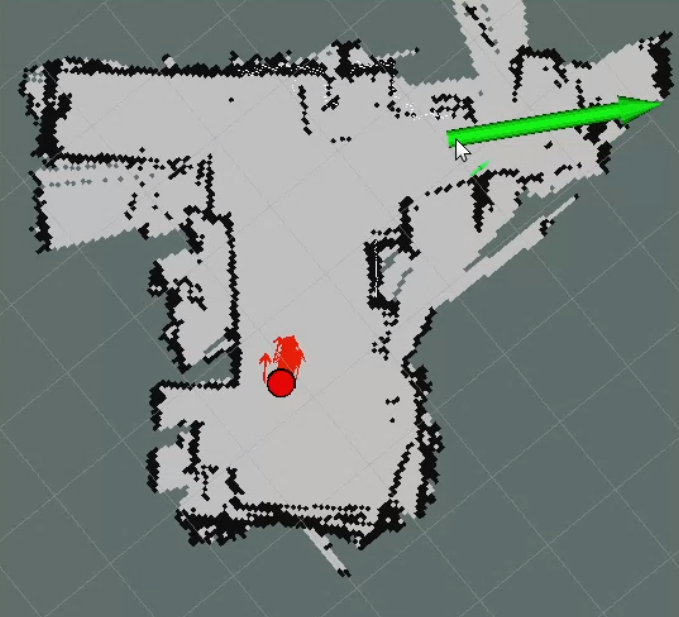
\includegraphics[scale=0.35]{./Figures/comando_navegacion.png}
    \caption{Captura de pantalla de RViz con el robot localizado al momento de recibir una orden de navegación.}
    \label{fig:comandoNavegación}
\end{figure}


\begin{figure}[ht]
    \centering
    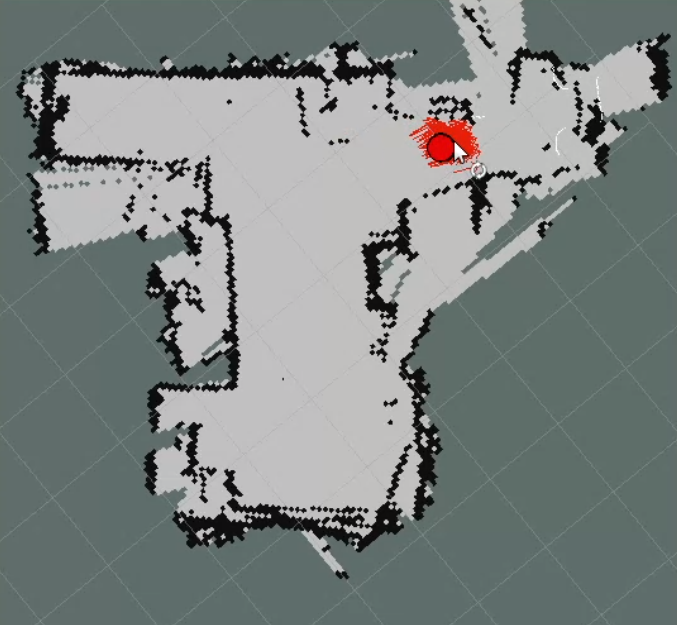
\includegraphics[scale=0.35]{./Figures/robot_en_setpoint.png}
    \caption{Captura de pantalla de RViz con el robot en su punto de consigna.}
    \label{fig:robotEnSetpoint}
\end{figure} 
%% !TEX root = ../memoria.tex

% Chapter Template

\chapter{Conclusiones} % Main chapter title

\label{Chapter5} % Change X to a consecutive number; for referencing this chapter elsewhere, use \ref{ChapterX}


%----------------------------------------------------------------------------------------

%----------------------------------------------------------------------------------------
%	SECTION 1
%----------------------------------------------------------------------------------------

\section{Conclusiones generales }

La idea de esta sección es resaltar cuáles son los principales aportes del trabajo realizado y cómo se podría continuar. Debe ser especialmente breve y concisa. Es buena idea usar un listado para enumerar los logros obtenidos.

Algunas preguntas que pueden servir para completar este capítulo:

\begin{itemize}
\item ¿Cuál es el grado de cumplimiento de los requerimientos?
\item ¿Cuán fielmente se puedo seguir la planificación original (cronograma incluido)?
\item ¿Se manifestó algunos de los riesgos identificados en la planificación? ¿Fue efectivo el plan de mitigación? ¿Se debió aplicar alguna otra acción no contemplada previamente?
\item Si se debieron hacer modificaciones a lo planificado ¿Cuáles fueron las causas y los efectos?
\item ¿Qué técnicas resultaron útiles para el desarrollo del proyecto y cuáles no tanto?
\end{itemize}


%----------------------------------------------------------------------------------------
%	SECTION 2
%----------------------------------------------------------------------------------------
\section{Próximos pasos}

Acá se indica cómo se podría continuar el trabajo más adelante.
 

%----------------------------------------------------------------------------------------
%	CONTENIDO DE LA MEMORIA  - APÉNDICES
%----------------------------------------------------------------------------------------

\appendix % indicativo para indicarle a LaTeX los siguientes "capítulos" son apéndices

% Incluir los apéndices de la memoria como archivos separadas desde la carpeta Appendices
% Descomentar las líneas a medida que se escriben los apéndices

%\include{Appendices/AppendixA}
%\include{Appendices/AppendixB}a
%\include{Appendices/AppendixC}

%----------------------------------------------------------------------------------------
%	BIBLIOGRAPHY
%----------------------------------------------------------------------------------------

\Urlmuskip=0mu plus 1mu\relax
\raggedright
\printbibliography[heading=bibintoc]

%----------------------------------------------------------------------------------------

\end{document}  
